% Options for packages loaded elsewhere
\PassOptionsToPackage{unicode}{hyperref}
\PassOptionsToPackage{hyphens}{url}
%
\documentclass[
]{article}
\usepackage{lmodern}
\usepackage{amsmath}
\usepackage{ifxetex,ifluatex}
\ifnum 0\ifxetex 1\fi\ifluatex 1\fi=0 % if pdftex
  \usepackage[T1]{fontenc}
  \usepackage[utf8]{inputenc}
  \usepackage{textcomp} % provide euro and other symbols
  \usepackage{amssymb}
\else % if luatex or xetex
  \usepackage{unicode-math}
  \defaultfontfeatures{Scale=MatchLowercase}
  \defaultfontfeatures[\rmfamily]{Ligatures=TeX,Scale=1}
\fi
% Use upquote if available, for straight quotes in verbatim environments
\IfFileExists{upquote.sty}{\usepackage{upquote}}{}
\IfFileExists{microtype.sty}{% use microtype if available
  \usepackage[]{microtype}
  \UseMicrotypeSet[protrusion]{basicmath} % disable protrusion for tt fonts
}{}
\makeatletter
\@ifundefined{KOMAClassName}{% if non-KOMA class
  \IfFileExists{parskip.sty}{%
    \usepackage{parskip}
  }{% else
    \setlength{\parindent}{0pt}
    \setlength{\parskip}{6pt plus 2pt minus 1pt}}
}{% if KOMA class
  \KOMAoptions{parskip=half}}
\makeatother
\usepackage{xcolor}
\IfFileExists{xurl.sty}{\usepackage{xurl}}{} % add URL line breaks if available
\IfFileExists{bookmark.sty}{\usepackage{bookmark}}{\usepackage{hyperref}}
\hypersetup{
  pdftitle={physiology\_stats},
  pdfauthor={Debbie Leung},
  hidelinks,
  pdfcreator={LaTeX via pandoc}}
\urlstyle{same} % disable monospaced font for URLs
\usepackage[margin=1in]{geometry}
\usepackage{color}
\usepackage{fancyvrb}
\newcommand{\VerbBar}{|}
\newcommand{\VERB}{\Verb[commandchars=\\\{\}]}
\DefineVerbatimEnvironment{Highlighting}{Verbatim}{commandchars=\\\{\}}
% Add ',fontsize=\small' for more characters per line
\usepackage{framed}
\definecolor{shadecolor}{RGB}{248,248,248}
\newenvironment{Shaded}{\begin{snugshade}}{\end{snugshade}}
\newcommand{\AlertTok}[1]{\textcolor[rgb]{0.94,0.16,0.16}{#1}}
\newcommand{\AnnotationTok}[1]{\textcolor[rgb]{0.56,0.35,0.01}{\textbf{\textit{#1}}}}
\newcommand{\AttributeTok}[1]{\textcolor[rgb]{0.77,0.63,0.00}{#1}}
\newcommand{\BaseNTok}[1]{\textcolor[rgb]{0.00,0.00,0.81}{#1}}
\newcommand{\BuiltInTok}[1]{#1}
\newcommand{\CharTok}[1]{\textcolor[rgb]{0.31,0.60,0.02}{#1}}
\newcommand{\CommentTok}[1]{\textcolor[rgb]{0.56,0.35,0.01}{\textit{#1}}}
\newcommand{\CommentVarTok}[1]{\textcolor[rgb]{0.56,0.35,0.01}{\textbf{\textit{#1}}}}
\newcommand{\ConstantTok}[1]{\textcolor[rgb]{0.00,0.00,0.00}{#1}}
\newcommand{\ControlFlowTok}[1]{\textcolor[rgb]{0.13,0.29,0.53}{\textbf{#1}}}
\newcommand{\DataTypeTok}[1]{\textcolor[rgb]{0.13,0.29,0.53}{#1}}
\newcommand{\DecValTok}[1]{\textcolor[rgb]{0.00,0.00,0.81}{#1}}
\newcommand{\DocumentationTok}[1]{\textcolor[rgb]{0.56,0.35,0.01}{\textbf{\textit{#1}}}}
\newcommand{\ErrorTok}[1]{\textcolor[rgb]{0.64,0.00,0.00}{\textbf{#1}}}
\newcommand{\ExtensionTok}[1]{#1}
\newcommand{\FloatTok}[1]{\textcolor[rgb]{0.00,0.00,0.81}{#1}}
\newcommand{\FunctionTok}[1]{\textcolor[rgb]{0.00,0.00,0.00}{#1}}
\newcommand{\ImportTok}[1]{#1}
\newcommand{\InformationTok}[1]{\textcolor[rgb]{0.56,0.35,0.01}{\textbf{\textit{#1}}}}
\newcommand{\KeywordTok}[1]{\textcolor[rgb]{0.13,0.29,0.53}{\textbf{#1}}}
\newcommand{\NormalTok}[1]{#1}
\newcommand{\OperatorTok}[1]{\textcolor[rgb]{0.81,0.36,0.00}{\textbf{#1}}}
\newcommand{\OtherTok}[1]{\textcolor[rgb]{0.56,0.35,0.01}{#1}}
\newcommand{\PreprocessorTok}[1]{\textcolor[rgb]{0.56,0.35,0.01}{\textit{#1}}}
\newcommand{\RegionMarkerTok}[1]{#1}
\newcommand{\SpecialCharTok}[1]{\textcolor[rgb]{0.00,0.00,0.00}{#1}}
\newcommand{\SpecialStringTok}[1]{\textcolor[rgb]{0.31,0.60,0.02}{#1}}
\newcommand{\StringTok}[1]{\textcolor[rgb]{0.31,0.60,0.02}{#1}}
\newcommand{\VariableTok}[1]{\textcolor[rgb]{0.00,0.00,0.00}{#1}}
\newcommand{\VerbatimStringTok}[1]{\textcolor[rgb]{0.31,0.60,0.02}{#1}}
\newcommand{\WarningTok}[1]{\textcolor[rgb]{0.56,0.35,0.01}{\textbf{\textit{#1}}}}
\usepackage{graphicx}
\makeatletter
\def\maxwidth{\ifdim\Gin@nat@width>\linewidth\linewidth\else\Gin@nat@width\fi}
\def\maxheight{\ifdim\Gin@nat@height>\textheight\textheight\else\Gin@nat@height\fi}
\makeatother
% Scale images if necessary, so that they will not overflow the page
% margins by default, and it is still possible to overwrite the defaults
% using explicit options in \includegraphics[width, height, ...]{}
\setkeys{Gin}{width=\maxwidth,height=\maxheight,keepaspectratio}
% Set default figure placement to htbp
\makeatletter
\def\fps@figure{htbp}
\makeatother
\setlength{\emergencystretch}{3em} % prevent overfull lines
\providecommand{\tightlist}{%
  \setlength{\itemsep}{0pt}\setlength{\parskip}{0pt}}
\setcounter{secnumdepth}{-\maxdimen} % remove section numbering
\ifluatex
  \usepackage{selnolig}  % disable illegal ligatures
\fi

\title{physiology\_stats}
\author{Debbie Leung}
\date{2/11/2021}

\begin{document}
\maketitle

\hypertarget{set-up}{%
\subsection{Set up}\label{set-up}}

\begin{Shaded}
\begin{Highlighting}[]
\CommentTok{\#install.packages("Hmisc")}
\FunctionTok{library}\NormalTok{(}\StringTok{"Hmisc"}\NormalTok{)}
\end{Highlighting}
\end{Shaded}

\begin{verbatim}
## Loading required package: lattice
\end{verbatim}

\begin{verbatim}
## Loading required package: survival
\end{verbatim}

\begin{verbatim}
## Loading required package: Formula
\end{verbatim}

\begin{verbatim}
## Loading required package: ggplot2
\end{verbatim}

\begin{verbatim}
## 
## Attaching package: 'Hmisc'
\end{verbatim}

\begin{verbatim}
## The following objects are masked from 'package:base':
## 
##     format.pval, units
\end{verbatim}

\begin{Shaded}
\begin{Highlighting}[]
\CommentTok{\#install.packages("corrplot")}
\FunctionTok{library}\NormalTok{(corrplot)}
\end{Highlighting}
\end{Shaded}

\begin{verbatim}
## corrplot 0.84 loaded
\end{verbatim}

\begin{Shaded}
\begin{Highlighting}[]
\FunctionTok{library}\NormalTok{(dplyr)}
\end{Highlighting}
\end{Shaded}

\begin{verbatim}
## 
## Attaching package: 'dplyr'
\end{verbatim}

\begin{verbatim}
## The following objects are masked from 'package:Hmisc':
## 
##     src, summarize
\end{verbatim}

\begin{verbatim}
## The following objects are masked from 'package:stats':
## 
##     filter, lag
\end{verbatim}

\begin{verbatim}
## The following objects are masked from 'package:base':
## 
##     intersect, setdiff, setequal, union
\end{verbatim}

\begin{Shaded}
\begin{Highlighting}[]
\FunctionTok{library}\NormalTok{(tidyr)}
\end{Highlighting}
\end{Shaded}

\begin{Shaded}
\begin{Highlighting}[]
\NormalTok{my\_data }\OtherTok{\textless{}{-}} \FunctionTok{read.csv}\NormalTok{(}\StringTok{"physiology\_cleaned.csv"}\NormalTok{, }\AttributeTok{stringsAsFactors =} \ConstantTok{FALSE}\NormalTok{) }\SpecialCharTok{\%\textgreater{}\%} \FunctionTok{na\_if}\NormalTok{(}\StringTok{""}\NormalTok{)}
\end{Highlighting}
\end{Shaded}

Steps: 1. Compute statistical tests 2. Compute normality and homogeneity
tests 3. Compute any post-hoc tests for significant results

\hypertarget{covariables-with-covariables}{%
\subsection{Covariables with
Covariables}\label{covariables-with-covariables}}

\hypertarget{correlation-matrix}{%
\subsubsection{Correlation Matrix}\label{correlation-matrix}}

Problem: cannot lump all continuous variables to display into a
correlation matrix because of missing NA values\ldots{} The matrices
computed below removed avg\_temp and temp\_sd.

\begin{Shaded}
\begin{Highlighting}[]
\NormalTok{con\_var\_na }\OtherTok{\textless{}{-}}\NormalTok{ my\_data }\SpecialCharTok{\%\textgreater{}\%} \FunctionTok{select}\NormalTok{(shell\_length}\SpecialCharTok{:}\NormalTok{heart\_rate)}
\NormalTok{test }\OtherTok{\textless{}{-}} \FunctionTok{cor}\NormalTok{(con\_var\_na, }\AttributeTok{use =} \StringTok{"complete.obs"}\NormalTok{, }\AttributeTok{method =} \FunctionTok{c}\NormalTok{(}\StringTok{"pearson"}\NormalTok{))}
\NormalTok{test}
\end{Highlighting}
\end{Shaded}

\begin{verbatim}
##                     shell_length average_weight weight_before weight_after
## shell_length          1.00000000     0.70127339    0.69882682   0.70356657
## average_weight        0.70127339     1.00000000    0.99987609   0.99987377
## weight_before         0.69882682     0.99987609    1.00000000   0.99949976
## weight_after          0.70356657     0.99987377    0.99949976   1.00000000
## weight_loss           0.05382386     0.28183940    0.29690809   0.26655924
## weight_loss_percent  -0.20152879    -0.09895452   -0.08358567  -0.11444196
## osmolality           -0.04749961     0.03115936    0.03459912   0.02767967
## heart_rate           -0.15731781    -0.20927667   -0.21004996  -0.20844357
##                     weight_loss weight_loss_percent  osmolality  heart_rate
## shell_length         0.05382386         -0.20152879 -0.04749961 -0.15731781
## average_weight       0.28183940         -0.09895452  0.03115936 -0.20927667
## weight_before        0.29690809         -0.08358567  0.03459912 -0.21004996
## weight_after         0.26655924         -0.11444196  0.02767967 -0.20844357
## weight_loss          1.00000000          0.90809698  0.21867101 -0.10769495
## weight_loss_percent  0.90809698          1.00000000  0.20236385 -0.07191950
## osmolality           0.21867101          0.20236385  1.00000000 -0.02903395
## heart_rate          -0.10769495         -0.07191950 -0.02903395  1.00000000
\end{verbatim}

\begin{Shaded}
\begin{Highlighting}[]
\CommentTok{\# cannot lump all continuous variables to display into a correlation matrix because of missing NA values... (cut out avg\_temp and temp\_sd)}
\NormalTok{con\_var }\OtherTok{\textless{}{-}}\NormalTok{ my\_data }\SpecialCharTok{\%\textgreater{}\%} \FunctionTok{select}\NormalTok{(shell\_length}\SpecialCharTok{:}\NormalTok{heart\_rate) }\SpecialCharTok{\%\textgreater{}\%}\NormalTok{ drop\_na}
\NormalTok{mydata.cor }\OtherTok{=} \FunctionTok{cor}\NormalTok{(con\_var, }\AttributeTok{method =} \FunctionTok{c}\NormalTok{(}\StringTok{"pearson"}\NormalTok{))}
\FunctionTok{corrplot}\NormalTok{(mydata.cor, }\AttributeTok{type =} \StringTok{"upper"}\NormalTok{, }\AttributeTok{order =} \StringTok{"hclust"}\NormalTok{, }\AttributeTok{tl.col =} \StringTok{"black"}\NormalTok{)}
\end{Highlighting}
\end{Shaded}

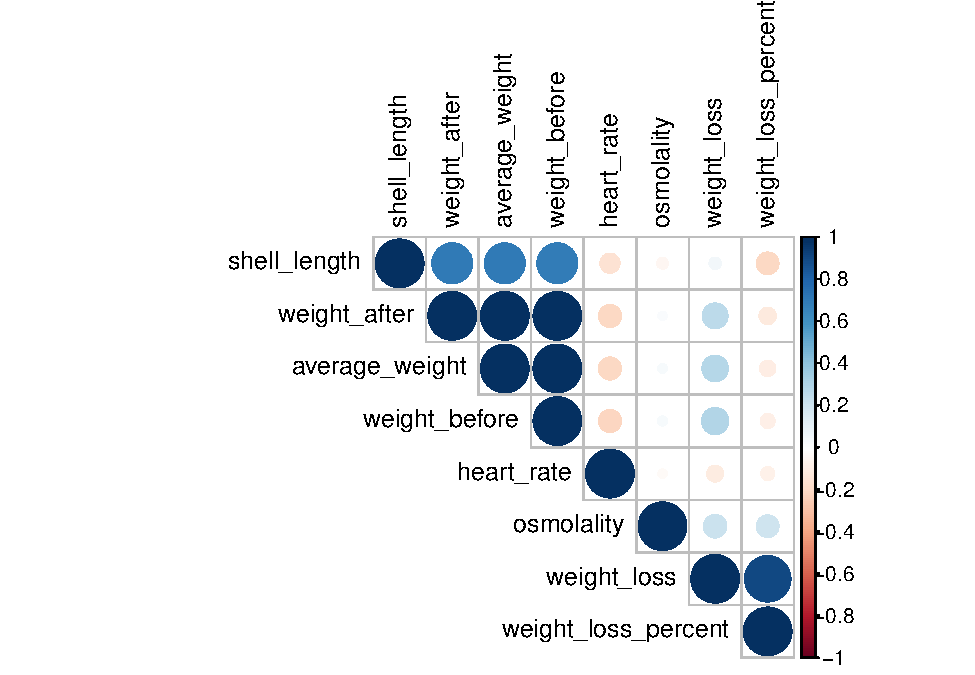
\includegraphics{physiology_stats_files/figure-latex/unnamed-chunk-4-1.pdf}

\begin{Shaded}
\begin{Highlighting}[]
\NormalTok{palette }\OtherTok{=} \FunctionTok{colorRampPalette}\NormalTok{(}\FunctionTok{c}\NormalTok{(}\StringTok{"blue"}\NormalTok{, }\StringTok{"white"}\NormalTok{, }\StringTok{"red"}\NormalTok{)) (}\DecValTok{20}\NormalTok{)}
\FunctionTok{heatmap}\NormalTok{(}\AttributeTok{x =}\NormalTok{ mydata.cor, }\AttributeTok{col =}\NormalTok{ palette, }\AttributeTok{symm =} \ConstantTok{TRUE}\NormalTok{)}
\end{Highlighting}
\end{Shaded}

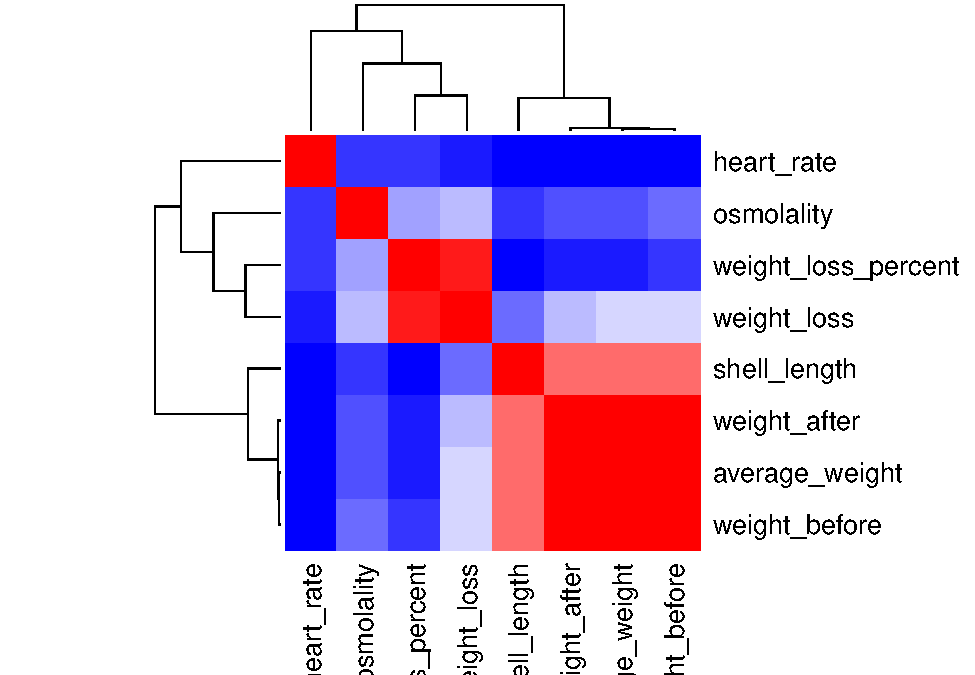
\includegraphics{physiology_stats_files/figure-latex/unnamed-chunk-4-2.pdf}

\begin{Shaded}
\begin{Highlighting}[]
\NormalTok{mydata.rcorr }\OtherTok{=} \FunctionTok{rcorr}\NormalTok{(}\FunctionTok{as.matrix}\NormalTok{(con\_var))}
\NormalTok{mydata.rcorr}
\end{Highlighting}
\end{Shaded}

\begin{verbatim}
##                     shell_length average_weight weight_before weight_after
## shell_length                1.00           0.70          0.70         0.70
## average_weight              0.70           1.00          1.00         1.00
## weight_before               0.70           1.00          1.00         1.00
## weight_after                0.70           1.00          1.00         1.00
## weight_loss                 0.05           0.28          0.30         0.27
## weight_loss_percent        -0.20          -0.10         -0.08        -0.11
## osmolality                 -0.05           0.03          0.03         0.03
## heart_rate                 -0.16          -0.21         -0.21        -0.21
##                     weight_loss weight_loss_percent osmolality heart_rate
## shell_length               0.05               -0.20      -0.05      -0.16
## average_weight             0.28               -0.10       0.03      -0.21
## weight_before              0.30               -0.08       0.03      -0.21
## weight_after               0.27               -0.11       0.03      -0.21
## weight_loss                1.00                0.91       0.22      -0.11
## weight_loss_percent        0.91                1.00       0.20      -0.07
## osmolality                 0.22                0.20       1.00      -0.03
## heart_rate                -0.11               -0.07      -0.03       1.00
## 
## n= 67 
## 
## 
## P
##                     shell_length average_weight weight_before weight_after
## shell_length                     0.0000         0.0000        0.0000      
## average_weight      0.0000                      0.0000        0.0000      
## weight_before       0.0000       0.0000                       0.0000      
## weight_after        0.0000       0.0000         0.0000                    
## weight_loss         0.6653       0.0209         0.0147        0.0292      
## weight_loss_percent 0.1020       0.4256         0.5013        0.3564      
## osmolality          0.7027       0.8023         0.7810        0.8240      
## heart_rate          0.2036       0.0892         0.0880        0.0905      
##                     weight_loss weight_loss_percent osmolality heart_rate
## shell_length        0.6653      0.1020              0.7027     0.2036    
## average_weight      0.0209      0.4256              0.8023     0.0892    
## weight_before       0.0147      0.5013              0.7810     0.0880    
## weight_after        0.0292      0.3564              0.8240     0.0905    
## weight_loss                     0.0000              0.0754     0.3857    
## weight_loss_percent 0.0000                          0.1005     0.5630    
## osmolality          0.0754      0.1005                         0.8156    
## heart_rate          0.3857      0.5630              0.8156
\end{verbatim}

\begin{Shaded}
\begin{Highlighting}[]
\FunctionTok{corrplot}\NormalTok{(mydata.rcorr}\SpecialCharTok{$}\NormalTok{r, }\AttributeTok{type=}\StringTok{"upper"}\NormalTok{, }\AttributeTok{order=}\StringTok{"hclust"}\NormalTok{, }\AttributeTok{tl.col =} \StringTok{"black"}\NormalTok{, }
         \AttributeTok{p.mat =}\NormalTok{ mydata.rcorr}\SpecialCharTok{$}\NormalTok{P, }\AttributeTok{sig.level =} \FloatTok{0.01}\NormalTok{, }\AttributeTok{insig =} \StringTok{"blank"}\NormalTok{)}
\end{Highlighting}
\end{Shaded}

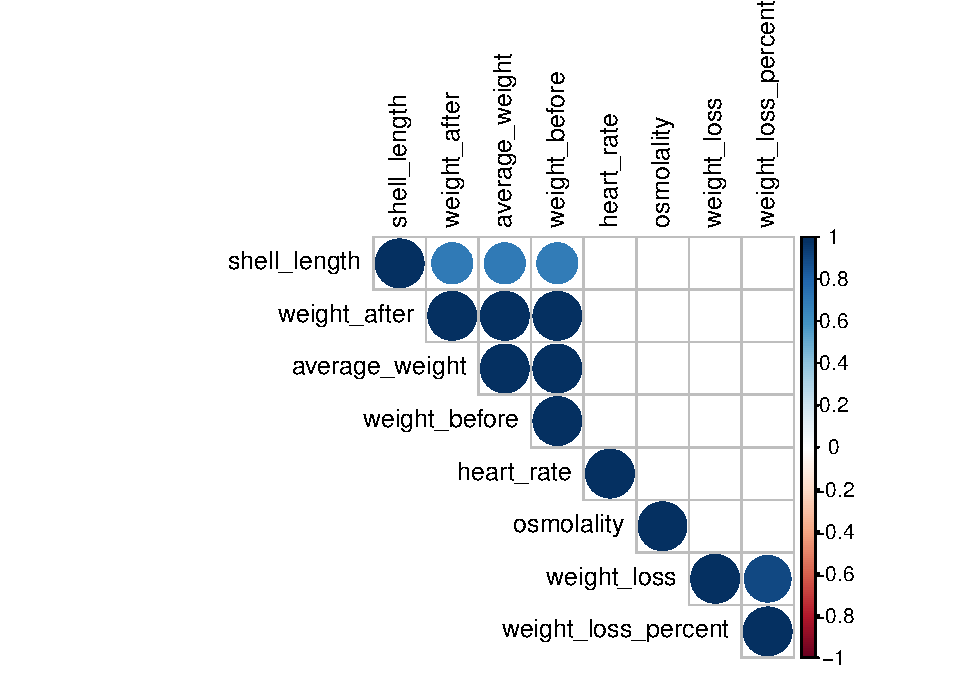
\includegraphics{physiology_stats_files/figure-latex/unnamed-chunk-5-1.pdf}

\begin{Shaded}
\begin{Highlighting}[]
\CommentTok{\# ++++++++++++++++++++++++++++}
\CommentTok{\# flattenCorrMatrix}
\CommentTok{\# ++++++++++++++++++++++++++++}
\CommentTok{\# cormat : matrix of the correlation coefficients}
\CommentTok{\# pmat : matrix of the correlation p{-}values}
\NormalTok{flattenCorrMatrix }\OtherTok{\textless{}{-}} \ControlFlowTok{function}\NormalTok{(cormat, pmat) \{}
\NormalTok{  ut }\OtherTok{\textless{}{-}} \FunctionTok{upper.tri}\NormalTok{(cormat)}
  \FunctionTok{data.frame}\NormalTok{(}
    \AttributeTok{row =} \FunctionTok{rownames}\NormalTok{(cormat)[}\FunctionTok{row}\NormalTok{(cormat)[ut]],}
    \AttributeTok{column =} \FunctionTok{rownames}\NormalTok{(cormat)[}\FunctionTok{col}\NormalTok{(cormat)[ut]],}
    \AttributeTok{cor  =}\NormalTok{(cormat)[ut],}
    \AttributeTok{p =}\NormalTok{ pmat[ut]}
\NormalTok{    )}
\NormalTok{\}}
\end{Highlighting}
\end{Shaded}

\begin{Shaded}
\begin{Highlighting}[]
\NormalTok{mydata.rcorr }\OtherTok{=} \FunctionTok{rcorr}\NormalTok{(}\FunctionTok{as.matrix}\NormalTok{(con\_var))}
\FunctionTok{flattenCorrMatrix}\NormalTok{(mydata.rcorr}\SpecialCharTok{$}\NormalTok{r, mydata.rcorr}\SpecialCharTok{$}\NormalTok{P)}
\end{Highlighting}
\end{Shaded}

\begin{verbatim}
##                    row              column         cor            p
## 1         shell_length      average_weight  0.70127339 3.872769e-11
## 2         shell_length       weight_before  0.69882682 4.833556e-11
## 3       average_weight       weight_before  0.99987609 0.000000e+00
## 4         shell_length        weight_after  0.70356657 3.139977e-11
## 5       average_weight        weight_after  0.99987377 0.000000e+00
## 6        weight_before        weight_after  0.99949976 0.000000e+00
## 7         shell_length         weight_loss  0.05382386 6.653126e-01
## 8       average_weight         weight_loss  0.28183940 2.085521e-02
## 9        weight_before         weight_loss  0.29690809 1.469317e-02
## 10        weight_after         weight_loss  0.26655924 2.922503e-02
## 11        shell_length weight_loss_percent -0.20152879 1.019720e-01
## 12      average_weight weight_loss_percent -0.09895452 4.256294e-01
## 13       weight_before weight_loss_percent -0.08358567 5.012776e-01
## 14        weight_after weight_loss_percent -0.11444196 3.564484e-01
## 15         weight_loss weight_loss_percent  0.90809698 0.000000e+00
## 16        shell_length          osmolality -0.04749961 7.026840e-01
## 17      average_weight          osmolality  0.03115936 8.023466e-01
## 18       weight_before          osmolality  0.03459912 7.810434e-01
## 19        weight_after          osmolality  0.02767967 8.240440e-01
## 20         weight_loss          osmolality  0.21867101 7.543688e-02
## 21 weight_loss_percent          osmolality  0.20236385 1.005305e-01
## 22        shell_length          heart_rate -0.15731781 2.035856e-01
## 23      average_weight          heart_rate -0.20927667 8.919805e-02
## 24       weight_before          heart_rate -0.21004996 8.799555e-02
## 25        weight_after          heart_rate -0.20844357 9.050798e-02
## 26         weight_loss          heart_rate -0.10769495 3.856908e-01
## 27 weight_loss_percent          heart_rate -0.07191950 5.630226e-01
## 28          osmolality          heart_rate -0.02903395 8.155829e-01
\end{verbatim}

\hypertarget{individual-pearson-correlation-tests}{%
\subsubsection{Individual Pearson Correlation
Tests}\label{individual-pearson-correlation-tests}}

\begin{Shaded}
\begin{Highlighting}[]
\FunctionTok{cor.test}\NormalTok{(my\_data}\SpecialCharTok{$}\NormalTok{average\_weight, my\_data}\SpecialCharTok{$}\NormalTok{shell\_length, }\AttributeTok{method =} \StringTok{"pearson"}\NormalTok{)}
\end{Highlighting}
\end{Shaded}

\begin{verbatim}
## 
##  Pearson's product-moment correlation
## 
## data:  my_data$average_weight and my_data$shell_length
## t = 7.7367, df = 76, p-value = 3.509e-11
## alternative hypothesis: true correlation is not equal to 0
## 95 percent confidence interval:
##  0.5177025 0.7722306
## sample estimates:
##       cor 
## 0.6637645
\end{verbatim}

Conclude body weight is positively correlated with shell length

\begin{Shaded}
\begin{Highlighting}[]
\CommentTok{\#Model\_1 \textless{}{-} lmer(trait1 \textasciitilde{} factor1, dataset)}
\CommentTok{\#anova(Model\_1, ddf="lme4")}
\end{Highlighting}
\end{Shaded}

\hypertarget{anova}{%
\subsubsection{ANOVA}\label{anova}}

Body weight, shell length, sex and experimental day are not statisically
significantly affected.

\begin{Shaded}
\begin{Highlighting}[]
\NormalTok{weight\_sex.aov }\OtherTok{\textless{}{-}} \FunctionTok{aov}\NormalTok{(average\_weight }\SpecialCharTok{\textasciitilde{}}\NormalTok{ sex, }\AttributeTok{data =}\NormalTok{ my\_data)}
\FunctionTok{summary}\NormalTok{(weight\_sex.aov)}
\end{Highlighting}
\end{Shaded}

\begin{verbatim}
##             Df Sum Sq Mean Sq F value Pr(>F)
## sex          2   8.65   4.325   2.374    0.1
## Residuals   75 136.66   1.822               
## 56 observations deleted due to missingness
\end{verbatim}

\begin{Shaded}
\begin{Highlighting}[]
\NormalTok{weight\_day.aov }\OtherTok{\textless{}{-}} \FunctionTok{aov}\NormalTok{(average\_weight }\SpecialCharTok{\textasciitilde{}}\NormalTok{ experimental\_day, }\AttributeTok{data =}\NormalTok{ my\_data)}
\FunctionTok{summary}\NormalTok{(weight\_day.aov)}
\end{Highlighting}
\end{Shaded}

\begin{verbatim}
##                  Df Sum Sq Mean Sq F value Pr(>F)
## experimental_day  3   5.93   1.977   1.049  0.376
## Residuals        74 139.39   1.884               
## 56 observations deleted due to missingness
\end{verbatim}

\begin{Shaded}
\begin{Highlighting}[]
\NormalTok{length\_sex.aov }\OtherTok{\textless{}{-}} \FunctionTok{aov}\NormalTok{(shell\_length }\SpecialCharTok{\textasciitilde{}}\NormalTok{ sex, }\AttributeTok{data =}\NormalTok{ my\_data)}
\FunctionTok{summary}\NormalTok{(length\_sex.aov)}
\end{Highlighting}
\end{Shaded}

\begin{verbatim}
##              Df Sum Sq Mean Sq F value Pr(>F)
## sex           2   16.5   8.256   1.119   0.33
## Residuals   131  966.3   7.377
\end{verbatim}

\begin{Shaded}
\begin{Highlighting}[]
\NormalTok{length\_day.aov }\OtherTok{\textless{}{-}} \FunctionTok{aov}\NormalTok{(shell\_length }\SpecialCharTok{\textasciitilde{}}\NormalTok{ experimental\_day, }\AttributeTok{data =}\NormalTok{ my\_data)}
\FunctionTok{summary}\NormalTok{(length\_day.aov)}
\end{Highlighting}
\end{Shaded}

\begin{verbatim}
##                   Df Sum Sq Mean Sq F value Pr(>F)
## experimental_day   4   31.2   7.796   1.057  0.381
## Residuals        129  951.7   7.377
\end{verbatim}

\hypertarget{covariables-with-dependent-variables}{%
\subsection{Covariables with Dependent
Variables}\label{covariables-with-dependent-variables}}

\hypertarget{correlation-tests}{%
\subsubsection{Correlation Tests}\label{correlation-tests}}

Please refer to the correlation matrix above. Below are individual tests
for body weight and dependent variables.

\begin{Shaded}
\begin{Highlighting}[]
\CommentTok{\#cor(x, method = "pearson", use = "complete.obs")}
\CommentTok{\#weight \textless{}{-} mydata[, c(7,8,12,13,14)] \%\textgreater{}\% drop\_na("osmolality")}
\end{Highlighting}
\end{Shaded}

\begin{Shaded}
\begin{Highlighting}[]
\FunctionTok{cor.test}\NormalTok{(my\_data}\SpecialCharTok{$}\NormalTok{average\_weight, my\_data}\SpecialCharTok{$}\NormalTok{weight\_loss, }\AttributeTok{method =} \StringTok{"pearson"}\NormalTok{)}
\end{Highlighting}
\end{Shaded}

\begin{verbatim}
## 
##  Pearson's product-moment correlation
## 
## data:  my_data$average_weight and my_data$weight_loss
## t = 2.1999, df = 75, p-value = 0.0309
## alternative hypothesis: true correlation is not equal to 0
## 95 percent confidence interval:
##  0.02351869 0.44560702
## sample estimates:
##       cor 
## 0.2462006
\end{verbatim}

Average weight is correlated with weight loss!!!

\begin{Shaded}
\begin{Highlighting}[]
\FunctionTok{cor.test}\NormalTok{(my\_data}\SpecialCharTok{$}\NormalTok{average\_weight, my\_data}\SpecialCharTok{$}\NormalTok{osmolality, }\AttributeTok{method =} \StringTok{"pearson"}\NormalTok{)}
\end{Highlighting}
\end{Shaded}

\begin{verbatim}
## 
##  Pearson's product-moment correlation
## 
## data:  my_data$average_weight and my_data$osmolality
## t = 0.42417, df = 75, p-value = 0.6727
## alternative hypothesis: true correlation is not equal to 0
## 95 percent confidence interval:
##  -0.1769983  0.2699410
## sample estimates:
##        cor 
## 0.04891993
\end{verbatim}

\begin{Shaded}
\begin{Highlighting}[]
\FunctionTok{cor.test}\NormalTok{(my\_data}\SpecialCharTok{$}\NormalTok{average\_weight, my\_data}\SpecialCharTok{$}\NormalTok{heart\_rate, }\AttributeTok{method =} \StringTok{"pearson"}\NormalTok{)}
\end{Highlighting}
\end{Shaded}

\begin{verbatim}
## 
##  Pearson's product-moment correlation
## 
## data:  my_data$average_weight and my_data$heart_rate
## t = -1.8031, df = 67, p-value = 0.07587
## alternative hypothesis: true correlation is not equal to 0
## 95 percent confidence interval:
##  -0.42991839  0.02270931
## sample estimates:
##        cor 
## -0.2151277
\end{verbatim}

\begin{Shaded}
\begin{Highlighting}[]
\FunctionTok{cor.test}\NormalTok{(my\_data}\SpecialCharTok{$}\NormalTok{average\_weight, my\_data}\SpecialCharTok{$}\NormalTok{average\_temp, }\AttributeTok{method =} \StringTok{"pearson"}\NormalTok{)}
\end{Highlighting}
\end{Shaded}

\begin{verbatim}
## 
##  Pearson's product-moment correlation
## 
## data:  my_data$average_weight and my_data$average_temp
## t = 0.47868, df = 2, p-value = 0.6794
## alternative hypothesis: true correlation is not equal to 0
## 95 percent confidence interval:
##  -0.9257242  0.9797903
## sample estimates:
##      cor 
## 0.320611
\end{verbatim}

\begin{Shaded}
\begin{Highlighting}[]
\FunctionTok{cor.test}\NormalTok{(my\_data}\SpecialCharTok{$}\NormalTok{average\_weight, my\_data}\SpecialCharTok{$}\NormalTok{temp\_sd, }\AttributeTok{method =} \StringTok{"pearson"}\NormalTok{)}
\end{Highlighting}
\end{Shaded}

\begin{verbatim}
## 
##  Pearson's product-moment correlation
## 
## data:  my_data$average_weight and my_data$temp_sd
## t = -0.31962, df = 2, p-value = 0.7796
## alternative hypothesis: true correlation is not equal to 0
## 95 percent confidence interval:
##  -0.9749687  0.9397421
## sample estimates:
##        cor 
## -0.2204467
\end{verbatim}

\hypertarget{manova}{%
\subsubsection{MANOVA}\label{manova}}

mshapiro.test( ){[}in the mvnormtest package{]} can be used to perform
the Shapiro-Wilk test for multivariate normality

\begin{Shaded}
\begin{Highlighting}[]
\NormalTok{res1\_sex.man }\OtherTok{\textless{}{-}} \FunctionTok{manova}\NormalTok{(}\FunctionTok{cbind}\NormalTok{(my\_data}\SpecialCharTok{$}\NormalTok{weight\_loss\_percent, my\_data}\SpecialCharTok{$}\NormalTok{osmolality, my\_data}\SpecialCharTok{$}\NormalTok{heart\_rate) }\SpecialCharTok{\textasciitilde{}}\NormalTok{ sex, }\AttributeTok{data =}\NormalTok{ my\_data)}
\FunctionTok{summary}\NormalTok{(res1\_sex.man)}
\end{Highlighting}
\end{Shaded}

\begin{verbatim}
##           Df Pillai approx F num Df den Df Pr(>F)
## sex        2 0.1269   1.4228      6    126 0.2109
## Residuals 64
\end{verbatim}

\begin{Shaded}
\begin{Highlighting}[]
\FunctionTok{summary.aov}\NormalTok{(res1\_sex.man)}
\end{Highlighting}
\end{Shaded}

\begin{verbatim}
##  Response 1 :
##             Df     Sum Sq    Mean Sq F value Pr(>F)
## sex          2 0.00014423 7.2114e-05  1.8845 0.1602
## Residuals   64 0.00244903 3.8266e-05               
## 
##  Response 2 :
##             Df Sum Sq Mean Sq F value Pr(>F)
## sex          2   9404  4702.1  1.9396 0.1521
## Residuals   64 155156  2424.3               
## 
##  Response 3 :
##             Df  Sum Sq   Mean Sq F value Pr(>F)
## sex          2 0.01437 0.0071845  1.3395 0.2692
## Residuals   64 0.34326 0.0053635               
## 
## 67 observations deleted due to missingness
\end{verbatim}

\begin{Shaded}
\begin{Highlighting}[]
\NormalTok{res2\_sex.man }\OtherTok{\textless{}{-}} \FunctionTok{manova}\NormalTok{(}\FunctionTok{cbind}\NormalTok{(my\_data}\SpecialCharTok{$}\NormalTok{average\_temp, my\_data}\SpecialCharTok{$}\NormalTok{temp\_sd) }\SpecialCharTok{\textasciitilde{}}\NormalTok{ sex, }\AttributeTok{data =}\NormalTok{ my\_data)}
\FunctionTok{summary}\NormalTok{(res2\_sex.man)}
\end{Highlighting}
\end{Shaded}

\begin{verbatim}
##           Df  Pillai approx F num Df den Df  Pr(>F)  
## sex        2 0.18665   2.9335      4    114 0.02374 *
## Residuals 57                                         
## ---
## Signif. codes:  0 '***' 0.001 '**' 0.01 '*' 0.05 '.' 0.1 ' ' 1
\end{verbatim}

\begin{Shaded}
\begin{Highlighting}[]
\FunctionTok{summary.aov}\NormalTok{(res2\_sex.man)}
\end{Highlighting}
\end{Shaded}

\begin{verbatim}
##  Response 1 :
##             Df Sum Sq Mean Sq F value  Pr(>F)  
## sex          2  71.38  35.691  2.7936 0.06959 .
## Residuals   57 728.22  12.776                  
## ---
## Signif. codes:  0 '***' 0.001 '**' 0.01 '*' 0.05 '.' 0.1 ' ' 1
## 
##  Response 2 :
##             Df Sum Sq Mean Sq F value Pr(>F)
## sex          2 0.4060 0.20301  1.8946 0.1597
## Residuals   57 6.1076 0.10715               
## 
## 74 observations deleted due to missingness
\end{verbatim}

Experimental day seems to have an effect on dependent variables\ldots{}

\begin{Shaded}
\begin{Highlighting}[]
\NormalTok{res1\_day.man }\OtherTok{\textless{}{-}} \FunctionTok{manova}\NormalTok{(}\FunctionTok{cbind}\NormalTok{(my\_data}\SpecialCharTok{$}\NormalTok{weight\_loss\_percent, my\_data}\SpecialCharTok{$}\NormalTok{osmolality, my\_data}\SpecialCharTok{$}\NormalTok{heart\_rate) }\SpecialCharTok{\textasciitilde{}}\NormalTok{ experimental\_day, }\AttributeTok{data =}\NormalTok{ my\_data)}
\FunctionTok{summary}\NormalTok{(res1\_day.man)}
\end{Highlighting}
\end{Shaded}

\begin{verbatim}
##                  Df  Pillai approx F num Df den Df    Pr(>F)    
## experimental_day  3 0.69418   6.3222      9    189 8.174e-08 ***
## Residuals        63                                             
## ---
## Signif. codes:  0 '***' 0.001 '**' 0.01 '*' 0.05 '.' 0.1 ' ' 1
\end{verbatim}

\begin{Shaded}
\begin{Highlighting}[]
\FunctionTok{summary.aov}\NormalTok{(res1\_day.man)}
\end{Highlighting}
\end{Shaded}

\begin{verbatim}
##  Response 1 :
##                  Df     Sum Sq    Mean Sq F value  Pr(>F)  
## experimental_day  3 0.00037924 1.2642e-04  3.5971 0.01824 *
## Residuals        63 0.00221401 3.5143e-05                  
## ---
## Signif. codes:  0 '***' 0.001 '**' 0.01 '*' 0.05 '.' 0.1 ' ' 1
## 
##  Response 2 :
##                  Df Sum Sq Mean Sq F value    Pr(>F)    
## experimental_day  3  78481 26160.4  19.146 6.139e-09 ***
## Residuals        63  86079  1366.3                      
## ---
## Signif. codes:  0 '***' 0.001 '**' 0.01 '*' 0.05 '.' 0.1 ' ' 1
## 
##  Response 3 :
##                  Df  Sum Sq   Mean Sq F value Pr(>F)
## experimental_day  3 0.00949 0.0031637  0.5725 0.6352
## Residuals        63 0.34814 0.0055261               
## 
## 67 observations deleted due to missingness
\end{verbatim}

\begin{Shaded}
\begin{Highlighting}[]
\NormalTok{res2\_day.man }\OtherTok{\textless{}{-}} \FunctionTok{manova}\NormalTok{(}\FunctionTok{cbind}\NormalTok{(my\_data}\SpecialCharTok{$}\NormalTok{average\_temp, my\_data}\SpecialCharTok{$}\NormalTok{temp\_sd) }\SpecialCharTok{\textasciitilde{}}\NormalTok{ experimental\_day, }\AttributeTok{data =}\NormalTok{ my\_data)}
\FunctionTok{summary}\NormalTok{(res2\_day.man)}
\end{Highlighting}
\end{Shaded}

\begin{verbatim}
##                  Df  Pillai approx F num Df den Df   Pr(>F)    
## experimental_day  1 0.32561   13.761      2     57 1.33e-05 ***
## Residuals        58                                            
## ---
## Signif. codes:  0 '***' 0.001 '**' 0.01 '*' 0.05 '.' 0.1 ' ' 1
\end{verbatim}

\begin{Shaded}
\begin{Highlighting}[]
\FunctionTok{summary.aov}\NormalTok{(res2\_day.man)}
\end{Highlighting}
\end{Shaded}

\begin{verbatim}
##  Response 1 :
##                  Df Sum Sq Mean Sq F value    Pr(>F)    
## experimental_day  1 243.11 243.111  25.338 4.973e-06 ***
## Residuals        58 556.50   9.595                      
## ---
## Signif. codes:  0 '***' 0.001 '**' 0.01 '*' 0.05 '.' 0.1 ' ' 1
## 
##  Response 2 :
##                  Df Sum Sq Mean Sq F value    Pr(>F)    
## experimental_day  1 1.9154 1.91542   24.16 7.627e-06 ***
## Residuals        58 4.5982 0.07928                      
## ---
## Signif. codes:  0 '***' 0.001 '**' 0.01 '*' 0.05 '.' 0.1 ' ' 1
## 
## 74 observations deleted due to missingness
\end{verbatim}

\hypertarget{independent-with-dependent}{%
\subsection{Independent with
Dependent}\label{independent-with-dependent}}

Questions: 1. Split tests based on the independent variables (3 factors)
or dependent variables (5 variables)? 2. How to best time point within
heating rate? 3. Do I need to do residual plots?

\begin{Shaded}
\begin{Highlighting}[]
\NormalTok{m\_weight }\OtherTok{\textless{}{-}} \FunctionTok{aov}\NormalTok{(my\_data}\SpecialCharTok{$}\NormalTok{weight\_loss\_percent }\SpecialCharTok{\textasciitilde{}}\NormalTok{ my\_data}\SpecialCharTok{$}\NormalTok{heating\_rate }\SpecialCharTok{*}\NormalTok{ my\_data}\SpecialCharTok{$}\NormalTok{tidal\_height }\SpecialCharTok{*}\NormalTok{ my\_data}\SpecialCharTok{$}\NormalTok{time\_point, }\AttributeTok{data =}\NormalTok{ my\_data)}
\FunctionTok{summary}\NormalTok{(m\_weight)}
\end{Highlighting}
\end{Shaded}

\begin{verbatim}
##                                                              Df    Sum Sq
## my_data$heating_rate                                          4 0.0015385
## my_data$tidal_height                                          1 0.0000009
## my_data$time_point                                            1 0.0003421
## my_data$heating_rate:my_data$tidal_height                     4 0.0000299
## my_data$heating_rate:my_data$time_point                       2 0.0000492
## my_data$tidal_height:my_data$time_point                       1 0.0000002
## my_data$heating_rate:my_data$tidal_height:my_data$time_point  2 0.0000109
## Residuals                                                    61 0.0012318
##                                                                Mean Sq F value
## my_data$heating_rate                                         0.0003846  19.048
## my_data$tidal_height                                         0.0000009   0.044
## my_data$time_point                                           0.0003421  16.942
## my_data$heating_rate:my_data$tidal_height                    0.0000075   0.370
## my_data$heating_rate:my_data$time_point                      0.0000246   1.219
## my_data$tidal_height:my_data$time_point                      0.0000002   0.010
## my_data$heating_rate:my_data$tidal_height:my_data$time_point 0.0000055   0.270
## Residuals                                                    0.0000202        
##                                                                Pr(>F)    
## my_data$heating_rate                                          3.3e-10 ***
## my_data$tidal_height                                         0.833943    
## my_data$time_point                                           0.000118 ***
## my_data$heating_rate:my_data$tidal_height                    0.829293    
## my_data$heating_rate:my_data$time_point                      0.302582    
## my_data$tidal_height:my_data$time_point                      0.922431    
## my_data$heating_rate:my_data$tidal_height:my_data$time_point 0.764051    
## Residuals                                                                
## ---
## Signif. codes:  0 '***' 0.001 '**' 0.01 '*' 0.05 '.' 0.1 ' ' 1
## 57 observations deleted due to missingness
\end{verbatim}

Need to further process to eliminate 3-way and 2-way interactions since
they are insiginificant?

\begin{Shaded}
\begin{Highlighting}[]
\NormalTok{m\_osmolality }\OtherTok{\textless{}{-}} \FunctionTok{aov}\NormalTok{(my\_data}\SpecialCharTok{$}\NormalTok{osmolality }\SpecialCharTok{\textasciitilde{}}\NormalTok{ my\_data}\SpecialCharTok{$}\NormalTok{heating\_rate }\SpecialCharTok{*}\NormalTok{ my\_data}\SpecialCharTok{$}\NormalTok{tidal\_height }\SpecialCharTok{*}\NormalTok{ my\_data}\SpecialCharTok{$}\NormalTok{time\_point, }\AttributeTok{data =}\NormalTok{ my\_data)}
\FunctionTok{summary}\NormalTok{(m\_osmolality)}
\end{Highlighting}
\end{Shaded}

\begin{verbatim}
##                                                              Df Sum Sq Mean Sq
## my_data$heating_rate                                          4  11758    2939
## my_data$tidal_height                                          1     64      64
## my_data$time_point                                            1   9152    9152
## my_data$heating_rate:my_data$tidal_height                     4   1249     312
## my_data$heating_rate:my_data$time_point                       2   9007    4503
## my_data$tidal_height:my_data$time_point                       1    361     361
## my_data$heating_rate:my_data$tidal_height:my_data$time_point  2   5866    2933
## Residuals                                                    61 148090    2428
##                                                              F value Pr(>F)  
## my_data$heating_rate                                           1.211 0.3155  
## my_data$tidal_height                                           0.026 0.8714  
## my_data$time_point                                             3.770 0.0568 .
## my_data$heating_rate:my_data$tidal_height                      0.129 0.9715  
## my_data$heating_rate:my_data$time_point                        1.855 0.1652  
## my_data$tidal_height:my_data$time_point                        0.149 0.7010  
## my_data$heating_rate:my_data$tidal_height:my_data$time_point   1.208 0.3058  
## Residuals                                                                    
## ---
## Signif. codes:  0 '***' 0.001 '**' 0.01 '*' 0.05 '.' 0.1 ' ' 1
## 57 observations deleted due to missingness
\end{verbatim}

\begin{Shaded}
\begin{Highlighting}[]
\NormalTok{m\_hr }\OtherTok{\textless{}{-}} \FunctionTok{aov}\NormalTok{(my\_data}\SpecialCharTok{$}\NormalTok{heart\_rate }\SpecialCharTok{\textasciitilde{}}\NormalTok{ my\_data}\SpecialCharTok{$}\NormalTok{heating\_rate }\SpecialCharTok{*}\NormalTok{ my\_data}\SpecialCharTok{$}\NormalTok{tidal\_height }\SpecialCharTok{*}\NormalTok{ my\_data}\SpecialCharTok{$}\NormalTok{time\_point, }\AttributeTok{data =}\NormalTok{ my\_data)}
\FunctionTok{summary}\NormalTok{(m\_hr)}
\end{Highlighting}
\end{Shaded}

\begin{verbatim}
##                                                              Df  Sum Sq
## my_data$heating_rate                                          4 0.08256
## my_data$tidal_height                                          1 0.00208
## my_data$time_point                                            1 0.02386
## my_data$heating_rate:my_data$tidal_height                     4 0.04694
## my_data$heating_rate:my_data$time_point                       2 0.00263
## my_data$tidal_height:my_data$time_point                       1 0.00005
## my_data$heating_rate:my_data$tidal_height:my_data$time_point  2 0.02109
## Residuals                                                    53 0.18207
##                                                               Mean Sq F value
## my_data$heating_rate                                         0.020641   6.008
## my_data$tidal_height                                         0.002083   0.606
## my_data$time_point                                           0.023860   6.945
## my_data$heating_rate:my_data$tidal_height                    0.011735   3.416
## my_data$heating_rate:my_data$time_point                      0.001317   0.384
## my_data$tidal_height:my_data$time_point                      0.000048   0.014
## my_data$heating_rate:my_data$tidal_height:my_data$time_point 0.010544   3.069
## Residuals                                                    0.003435        
##                                                                Pr(>F)    
## my_data$heating_rate                                         0.000461 ***
## my_data$tidal_height                                         0.439597    
## my_data$time_point                                           0.010996 *  
## my_data$heating_rate:my_data$tidal_height                    0.014742 *  
## my_data$heating_rate:my_data$time_point                      0.683346    
## my_data$tidal_height:my_data$time_point                      0.906228    
## my_data$heating_rate:my_data$tidal_height:my_data$time_point 0.054797 .  
## Residuals                                                                
## ---
## Signif. codes:  0 '***' 0.001 '**' 0.01 '*' 0.05 '.' 0.1 ' ' 1
## 65 observations deleted due to missingness
\end{verbatim}

\begin{Shaded}
\begin{Highlighting}[]
\NormalTok{m\_atemp }\OtherTok{\textless{}{-}} \FunctionTok{aov}\NormalTok{(my\_data}\SpecialCharTok{$}\NormalTok{average\_temp }\SpecialCharTok{\textasciitilde{}}\NormalTok{ my\_data}\SpecialCharTok{$}\NormalTok{heating\_rate }\SpecialCharTok{*}\NormalTok{ my\_data}\SpecialCharTok{$}\NormalTok{tidal\_height }\SpecialCharTok{*}\NormalTok{ my\_data}\SpecialCharTok{$}\NormalTok{time\_point, }\AttributeTok{data =}\NormalTok{ my\_data)}
\FunctionTok{summary}\NormalTok{(m\_atemp)}
\end{Highlighting}
\end{Shaded}

\begin{verbatim}
##                                                              Df Sum Sq Mean Sq
## my_data$heating_rate                                          4  722.0  180.50
## my_data$tidal_height                                          1    0.6    0.56
## my_data$time_point                                            1   11.8   11.80
## my_data$heating_rate:my_data$tidal_height                     4    7.9    1.98
## my_data$heating_rate:my_data$time_point                       2    6.5    3.26
## my_data$tidal_height:my_data$time_point                       1    0.0    0.01
## my_data$heating_rate:my_data$tidal_height:my_data$time_point  2    1.3    0.65
## Residuals                                                    44   49.5    1.12
##                                                              F value  Pr(>F)
## my_data$heating_rate                                         160.514 < 2e-16
## my_data$tidal_height                                           0.499 0.48385
## my_data$time_point                                            10.494 0.00228
## my_data$heating_rate:my_data$tidal_height                      1.761 0.15391
## my_data$heating_rate:my_data$time_point                        2.900 0.06562
## my_data$tidal_height:my_data$time_point                        0.012 0.91379
## my_data$heating_rate:my_data$tidal_height:my_data$time_point   0.574 0.56726
## Residuals                                                                   
##                                                                 
## my_data$heating_rate                                         ***
## my_data$tidal_height                                            
## my_data$time_point                                           ** 
## my_data$heating_rate:my_data$tidal_height                       
## my_data$heating_rate:my_data$time_point                      .  
## my_data$tidal_height:my_data$time_point                         
## my_data$heating_rate:my_data$tidal_height:my_data$time_point    
## Residuals                                                       
## ---
## Signif. codes:  0 '***' 0.001 '**' 0.01 '*' 0.05 '.' 0.1 ' ' 1
## 74 observations deleted due to missingness
\end{verbatim}

\begin{Shaded}
\begin{Highlighting}[]
\NormalTok{m\_tempsd }\OtherTok{\textless{}{-}} \FunctionTok{aov}\NormalTok{(my\_data}\SpecialCharTok{$}\NormalTok{temp\_sd }\SpecialCharTok{\textasciitilde{}}\NormalTok{ my\_data}\SpecialCharTok{$}\NormalTok{heating\_rate }\SpecialCharTok{*}\NormalTok{ my\_data}\SpecialCharTok{$}\NormalTok{tidal\_height }\SpecialCharTok{*}\NormalTok{ my\_data}\SpecialCharTok{$}\NormalTok{time\_point, }\AttributeTok{data =}\NormalTok{ my\_data)}
\FunctionTok{summary}\NormalTok{(m\_tempsd)}
\end{Highlighting}
\end{Shaded}

\begin{verbatim}
##                                                              Df Sum Sq Mean Sq
## my_data$heating_rate                                          4  4.915  1.2289
## my_data$tidal_height                                          1  0.009  0.0091
## my_data$time_point                                            1  0.001  0.0009
## my_data$heating_rate:my_data$tidal_height                     4  0.252  0.0629
## my_data$heating_rate:my_data$time_point                       2  0.015  0.0075
## my_data$tidal_height:my_data$time_point                       1  0.090  0.0904
## my_data$heating_rate:my_data$tidal_height:my_data$time_point  2  0.189  0.0946
## Residuals                                                    44  1.042  0.0237
##                                                              F value  Pr(>F)
## my_data$heating_rate                                          51.893 4.2e-16
## my_data$tidal_height                                           0.386  0.5377
## my_data$time_point                                             0.038  0.8467
## my_data$heating_rate:my_data$tidal_height                      2.657  0.0452
## my_data$heating_rate:my_data$time_point                        0.316  0.7309
## my_data$tidal_height:my_data$time_point                        3.816  0.0571
## my_data$heating_rate:my_data$tidal_height:my_data$time_point   3.994  0.0255
## Residuals                                                                   
##                                                                 
## my_data$heating_rate                                         ***
## my_data$tidal_height                                            
## my_data$time_point                                              
## my_data$heating_rate:my_data$tidal_height                    *  
## my_data$heating_rate:my_data$time_point                         
## my_data$tidal_height:my_data$time_point                      .  
## my_data$heating_rate:my_data$tidal_height:my_data$time_point *  
## Residuals                                                       
## ---
## Signif. codes:  0 '***' 0.001 '**' 0.01 '*' 0.05 '.' 0.1 ' ' 1
## 74 observations deleted due to missingness
\end{verbatim}

\hypertarget{references}{%
\subsection{References}\label{references}}

\begin{itemize}
\tightlist
\item
  correlation matrix:
  \url{http://www.sthda.com/english/wiki/correlation-matrix-a-quick-start-guide-to-analyze-format-and-visualize-a-correlation-matrix-using-r-software}
\item
  three-way ANOVA:
  \url{https://www.r-bloggers.com/2017/02/raccoon-ch-2-4-3-way-anova/}
\end{itemize}

\end{document}
